\subsection{Problemas de información repetida}

Dentro de los problemas de información repetida, para guardar la información, juntamos aquellas clases que provenían del mismo grupo. A continuación presentamos los casos que encontramos con el problema de tener información repetida.

\begin{itemize}
\item[-] El número del plan de estudios corresponde al año en que entró en vigencia el plan. Por ejemplo, si se tiene un plan 2015 en Actuaría, entonces dicho plan comenzó a tener vigencia a partir del año 2015. Debido a ésto no debería de existir un horario con un plan posterior al año del semestre.

En la subfigura $(a)$ de la \figurename{~\ref{planRepetido}} podemos ver una materia de la carrera de Ciencias de la Computación del semestre 2008-2, con el plan 2013, lo cual no es cronológicamente correcto:

\url{http://www.fciencias.unam.mx/docencia/horarios/20082/1556/803}.

En la subfigura $(b)$ de la misma figura, vemos la información de la misma materia y del mismo grupo pero con el plan 1994:

\url{http://www.fciencias.unam.mx/docencia/horarios/20082/218/803}.

\begin{figure}[H]
\centering
\subfigure[\textit{Plan de estudios posterior}]{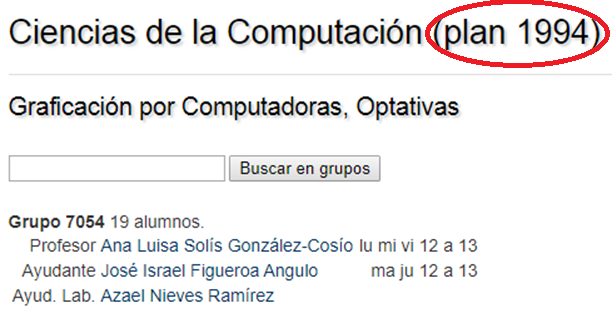
\includegraphics[width=11cm]{InfoRepetida_A_1}} %%Ping\"uino %%[angle=30]
	\subfigure[\textit{Plan de estudios correspondiente}]{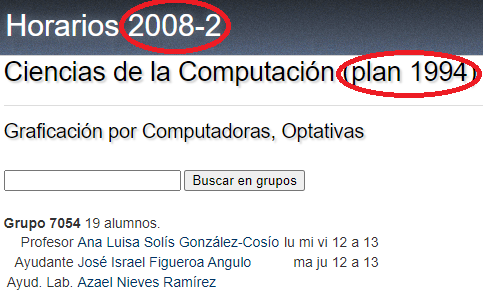
\includegraphics[width=11cm]{InfoRepetida_A_2}}
	\caption[\textit{Información repetida: Planes de estudio}]{\textit{Se muestra un ejemplo de información repetida por los planes de estudio. No deberían de existir grupos con planes posteriores al año del semestre en el que se busca información.}}\label{planRepetido}
\end{figure}

\item[-] Encontramos grupos correspondientes a una misma materia con nombres distintos para diferentes carreras.

En la subfigura $(a)$ de la \figurename{~\ref{MateriaNombresDistintos}} vemos un ejemplo con la información de la materia \textit{Estadística III}, para la carrera de Matemáticas plan 1983: \url{http://www.fciencias.unam.mx/docencia/horarios/20201/217/1712}.

En la subfigura $(b)$ de la figura mencionada se muestra la información de la materia \textit{Modelos de Superviciencia y de Series de Tiempo}, para la carrera de Actuaría plan 2015: \url{http://www.fciencias.unam.mx/docencia/horarios/20201/2017/1739}.

Notamos que la información en ambos ejemplos es la misma. Sólo cambian las claves de los grupos y el nombre de las materias. Cabe mencionar que ambas páginas corresponden al semestre 2020-1.

\begin{figure}[H]
	\centering
	\subfigure[\textit{Matemáticas plan 1983}]{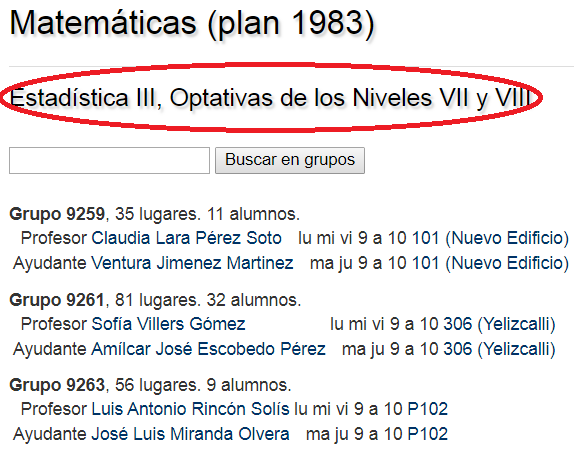
\includegraphics[width=11cm]{InfoRepetida_B_1}} %%Ping\"uino %%[angle=30]
	\subfigure[\textit{Actuaría plan 2015}]{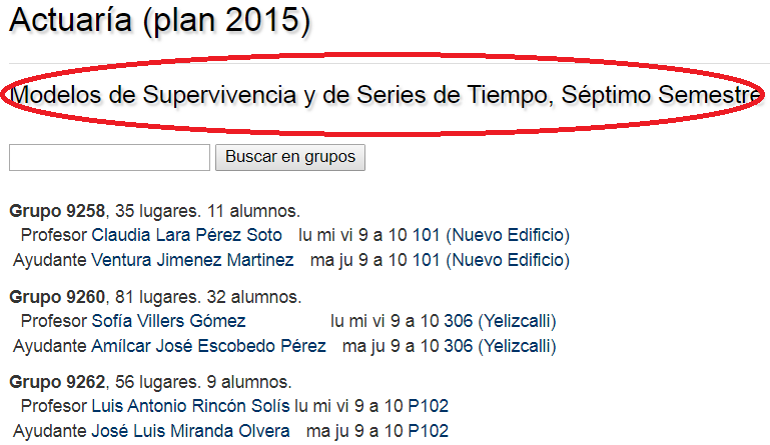
\includegraphics[width=14cm]{InfoRepetida_B_2}}
	\caption[\textit{Información repetida: Materia con nombres distintos}]{\textit{Se muestra un ejemplo de información repetida por materia con nombres distintos. En estos casos se tienen materias que tienen nombres diferentes de acuerdo a la carrera o plan de estudios.}}\label{MateriaNombresDistintos}
\end{figure}

\item[-] Encontramos grupos con profesores que imparten dos o más clases distintas en el mismo horario y diferente salón.

En la subfigura $(a)$ de la \figurename{~\ref{UnProfMuchasMaterias}} se observa un ejemplo con la información de la materia \textit{Ecuaciones Diferenciales I}, del semestre 2011-1: \url{http://www.fciencias.unam.mx/docencia/horarios/20111/2017/162}.

En la subfigura $(b)$ de la figura mencionada se muestra la información de la materia \textit{Cálculo Diferencial e Integral I}, del semestre 2011-1: \url{http://www.fciencias.unam.mx/docencia/horarios/20111/2017/91}.

Las materias mencionadas son diferentes, pero las clases comienzan a la misma hora, \textit{Ecuaciones Diferenciales I} de 18-19hrs y \textit{Cálculo Diferencial e Integral I} de 18-20hrs. Dado que se tiene la misma ayudante pudiera ser que se intercambien las horas, pero no se puede asignar más de una clase a la misma hora al mismo profesor.

%EJEMPLO CON PROFESOR: Bartolo Guzmán Guevara
%Ecuaciones Diferenciales Parciales II
%\url{http://www.fciencias.unam.mx/docencia/horarios/20131/217/183}
%\url{http://www.fciencias.unam.mx/docencia/horarios/20131/119/183}
%\url{http://www.fciencias.unam.mx/docencia/horarios/20131/2055/183}
%Matemáticas Avanzadas de la Física
%\url{http://www.fciencias.unam.mx/docencia/horarios/20131/217/610}
%Funciones Especiales y Transformadas Integrales
%\url{http://www.fciencias.unam.mx/docencia/horarios/20131/218/217}
%\url{http://www.fciencias.unam.mx/docencia/horarios/20131/119/217}

%EJEMPLO CON PROFESORA: Tania Eréndira Rivera Torres. Introducción Matemática a la Mecánica Celeste y Álgebra Lineal I
%http://www.fciencias.unam.mx/docencia/horarios/20082/119/5
%http://www.fciencias.unam.mx/docencia/horarios/20082/119/356
%http://www.fciencias.unam.mx/docencia/horarios/20082/1176/5
%http://www.fciencias.unam.mx/docencia/horarios/20082/2017/5
%http://www.fciencias.unam.mx/docencia/horarios/20082/218/5
%http://www.fciencias.unam.mx/docencia/horarios/20082/1556/5
%http://www.fciencias.unam.mx/docencia/horarios/20082/217/5
%http://www.fciencias.unam.mx/docencia/horarios/20082/217/356
%http://www.fciencias.unam.mx/docencia/horarios/20082/2055/5 

%EJEMPLO CON PROFESOR: Hugo Alberto Rincón Mejía. Álgebra Moderna II y Álgebra Moderna III
%http://www.fciencias.unam.mx/docencia/horarios/20192/119/2
%http://www.fciencias.unam.mx/docencia/horarios/20081/119/3
%http://www.fciencias.unam.mx/docencia/horarios/20192/218/2
%http://www.fciencias.unam.mx/docencia/horarios/20192/1556/2
%http://www.fciencias.unam.mx/docencia/horarios/20192/217/2

%EJEMPLO CON PROFESOR: Roberto Pichardo Mendoza. Seminario de Apoyo a la Titulación en Matemáticas A y Geometría Analítica II
%http://www.fciencias.unam.mx/docencia/horarios/20192/119/245
%http://www.fciencias.unam.mx/docencia/horarios/20192/1176/245
%http://www.fciencias.unam.mx/docencia/horarios/20192/2017/245
%http://www.fciencias.unam.mx/docencia/horarios/20192/218/245
%http://www.fciencias.unam.mx/docencia/horarios/20192/217/245
%http://www.fciencias.unam.mx/docencia/horarios/20192/217/959
%http://www.fciencias.unam.mx/docencia/horarios/20192/2055/245

%EJEMPLO CON PROFESOR: Roberto Pichardo Mendoza. Seminario de Topología A y Seminario de Apoyo a la Titulación en Matemáticas A
%http://www.fciencias.unam.mx/docencia/horarios/20191/119/977
%http://www.fciencias.unam.mx/docencia/horarios/20191/217/959
%http://www.fciencias.unam.mx/docencia/horarios/20191/217/977

%EJEMPLO CON PROFESOR: Sergio Iván López Ortega. Probabilidad II y Procesos Estocásticos II
%http://www.fciencias.unam.mx/docencia/horarios/20112/119/626
%http://www.fciencias.unam.mx/docencia/horarios/20112/119/631
%http://www.fciencias.unam.mx/docencia/horarios/20112/1176/626
%http://www.fciencias.unam.mx/docencia/horarios/20112/1176/631
%http://www.fciencias.unam.mx/docencia/horarios/20112/2017/626
%http://www.fciencias.unam.mx/docencia/horarios/20112/2017/631
%http://www.fciencias.unam.mx/docencia/horarios/20112/218/626
%http://www.fciencias.unam.mx/docencia/horarios/20112/1556/626
%http://www.fciencias.unam.mx/docencia/horarios/20112/217/626
%http://www.fciencias.unam.mx/docencia/horarios/20112/217/631
%http://www.fciencias.unam.mx/docencia/horarios/20112/2055/626
%http://www.fciencias.unam.mx/docencia/horarios/20112/2055/631

%EJEMPLO CON PROFESORA: Ana Patricia Kuri González. Seminario sobre Enseñanza de las Matemáticas II y Seminario sobre Enseñanza de las Matemáticas I
%http://www.fciencias.unam.mx/docencia/horarios/20172/119/751
%http://www.fciencias.unam.mx/docencia/horarios/20172/119/754
%http://www.fciencias.unam.mx/docencia/horarios/20172/218/751
%http://www.fciencias.unam.mx/docencia/horarios/20172/218/754
%http://www.fciencias.unam.mx/docencia/horarios/20172/217/751
%http://www.fciencias.unam.mx/docencia/horarios/20172/217/754

%EJEMPLO CON PROFESORA: Tania Eréndira Rivera Torres. Introducción Matemática a la Mecánica Celeste y Álgebra Lineal I
%http://www.fciencias.unam.mx/docencia/horarios/20082/119/5
%http://www.fciencias.unam.mx/docencia/horarios/20082/119/356
%http://www.fciencias.unam.mx/docencia/horarios/20082/1176/5
%http://www.fciencias.unam.mx/docencia/horarios/20082/2017/5
%http://www.fciencias.unam.mx/docencia/horarios/20082/218/5
%http://www.fciencias.unam.mx/docencia/horarios/20082/1556/5
%http://www.fciencias.unam.mx/docencia/horarios/20082/217/5
%http://www.fciencias.unam.mx/docencia/horarios/20082/217/356
%http://www.fciencias.unam.mx/docencia/horarios/20082/2055/5

%EJEMPLO CON PROFESOR: Juan Rivera Alcántara. Teoría del Riesgo y Valuación de Opciones
%http://www.fciencias.unam.mx/docencia/horarios/20082/119/1067
%http://www.fciencias.unam.mx/docencia/horarios/20082/119/1807
%http://www.fciencias.unam.mx/docencia/horarios/20082/1176/1067
%http://www.fciencias.unam.mx/docencia/horarios/20082/1176/1807
%http://www.fciencias.unam.mx/docencia/horarios/20082/2017/1807

%EJEMPLO CON PROFESOR: Javier Valdez Quijada. Teoría de los Números I y Teoría de los Números II
%http://www.fciencias.unam.mx/docencia/horarios/20172/119/764
%http://www.fciencias.unam.mx/docencia/horarios/20172/119/777
%http://www.fciencias.unam.mx/docencia/horarios/20172/218/764
%http://www.fciencias.unam.mx/docencia/horarios/20172/218/777
%http://www.fciencias.unam.mx/docencia/horarios/20172/1556/764
%http://www.fciencias.unam.mx/docencia/horarios/20172/1556/777
%http://www.fciencias.unam.mx/docencia/horarios/20172/217/764
%http://www.fciencias.unam.mx/docencia/horarios/20172/217/777


\begin{figure}[H]
	\centering
	\subfigure[\textit{Ecuaciones Diferenciales I}]{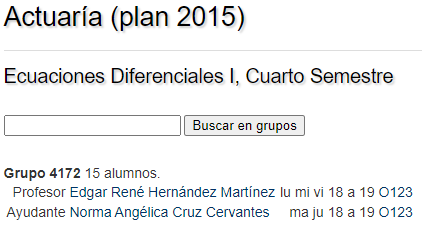
\includegraphics[width=10cm]{Ej_gpo_repetido_1}} %%Ping\"uino %%[angle=30]
	\subfigure[\textit{Cálculo Diferencial e Integral I}]{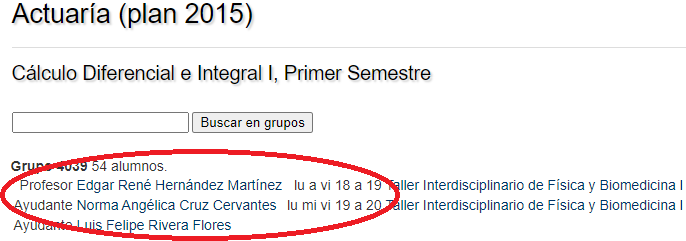
\includegraphics[width=15cm]{Ej_gpo_repetido_2}}
	\caption[\textit{Información repetida: Mismo profesor, misma hora, materias distintas}]{\textit{Se muestra un ejemplo de información repetida por tener un mismo profesor impartiendo materias distintas, en distinto salón, a la misma hora.}}\label{UnProfMuchasMaterias}
\end{figure}	

\end{itemize}
